\documentclass[12pt, a4]{article}
\usepackage[english]{babel}
\usepackage[utf8x]{inputenc}
\usepackage{fullpage}
\usepackage{listings}
\usepackage{graphicx}
\usepackage{color}

%Syntax highlighting
\definecolor{blue-violet}{rgb}{0.54, 0.17, 0.89}
\definecolor{ao}{rgb}{0.0, 0.5, 0.0}
\definecolor{amaranth}{rgb}{0.9, 0.17, 0.31}
\definecolor{ballblue}{rgb}{0.13, 0.67, 0.8}
\definecolor{onyx}{rgb}{0.06, 0.06, 0.06}


\lstset{
  breaklines=true,                 % automatic line breaking only at whitespace
  captionpos=b,                    % sets the caption-position to bottom
  breakatwhitespace=false,
  keepspaces=true,
  numbers=left,
  numbersep=5pt,
  showspaces=false,
  showstringspaces=false,
  showtabs=false,
  tabsize=4,  
  backgroundcolor=\color{white},   % choose the background color
  commentstyle=\color{ao},    % comment style
  keywordstyle=\color{amaranth},    % keyword style
  stringstyle=\color{blue-violet},    % string literal style
  numberstyle=\tiny\color{ballblue},	   % number style
  basicstyle=\ttfamily\footnotesize\color{onyx} % size of fonts used for the code
}

%Document Header
\title{\textbf{Department of CSE\\SSN College of Engineering}}
\author{\textbf{Vishakan Subramanian - 18 5001 196 - Semester VI}}
\date{3 February 2021}

\begin{document}
\maketitle
\hrule
\section*{\center{UCS 1611 - Internet Programming Lab}}
\hrule
\bigskip

%Assignment Details
\subsection*{\center{\textbf{Exercise 1: Website for International Conference Using HTML5 Tags}}}
\subsection*{\flushleft{Learning Objective:}}
\begin{flushleft}
To develop a Website for an International Conference using \textbf{HTML5 elements} with the following specifications:-

\begin{itemize}
\item The conference homepage should consists of the following tabs:
Home, Committee, Call For Papers, Important Dates, Workshops,
Registration and Contact.
\item On clicking each tab, it should open in a separate page.
\item The website should contain background Image, logos, header, footer.
\item Use tooltip text for help.
\item For pre-conference workshop registration use form elements.
\item Mandatory Tags: List, Table, Anchor, Image, Semantic Tags.
\end{itemize}
 
\end{flushleft}

%Code
\newpage
\subsection*{\flushleft{Code - Home Page:}}
\begin{flushleft}
\lstinputlisting[language = HTML]{index.html}
\end{flushleft}

\newpage
\subsection*{\flushleft{Code - Committee Page:}}
\begin{flushleft}
\lstinputlisting[language = HTML]{committee.html}
\end{flushleft}

\newpage
\subsection*{\flushleft{Code - Call for Papers Page:}}
\begin{flushleft}
\lstinputlisting[language = HTML]{papers.html}
\end{flushleft}

\newpage
\subsection*{\flushleft{Code - Important Dates Page:}}
\begin{flushleft}
\lstinputlisting[language = HTML]{dates.html}
\end{flushleft}

\newpage
\subsection*{\flushleft{Code - Workshops Page:}}
\begin{flushleft}
\lstinputlisting[language = HTML]{workshops.html}
\end{flushleft}

\newpage
\subsection*{\flushleft{Code - Registration Page:}}
\begin{flushleft}
\lstinputlisting[language = HTML]{reg.html}
\end{flushleft}

\newpage
\subsection*{\flushleft{Code - Contact Page:}}
\begin{flushleft}
\lstinputlisting[language = HTML]{contact.html}
\end{flushleft}

%Output
\newpage
\subsection*{\flushleft{Output - Home Page:}}
\begin{figure}[h]
\centering
\caption{Browser Output: Home Page.}
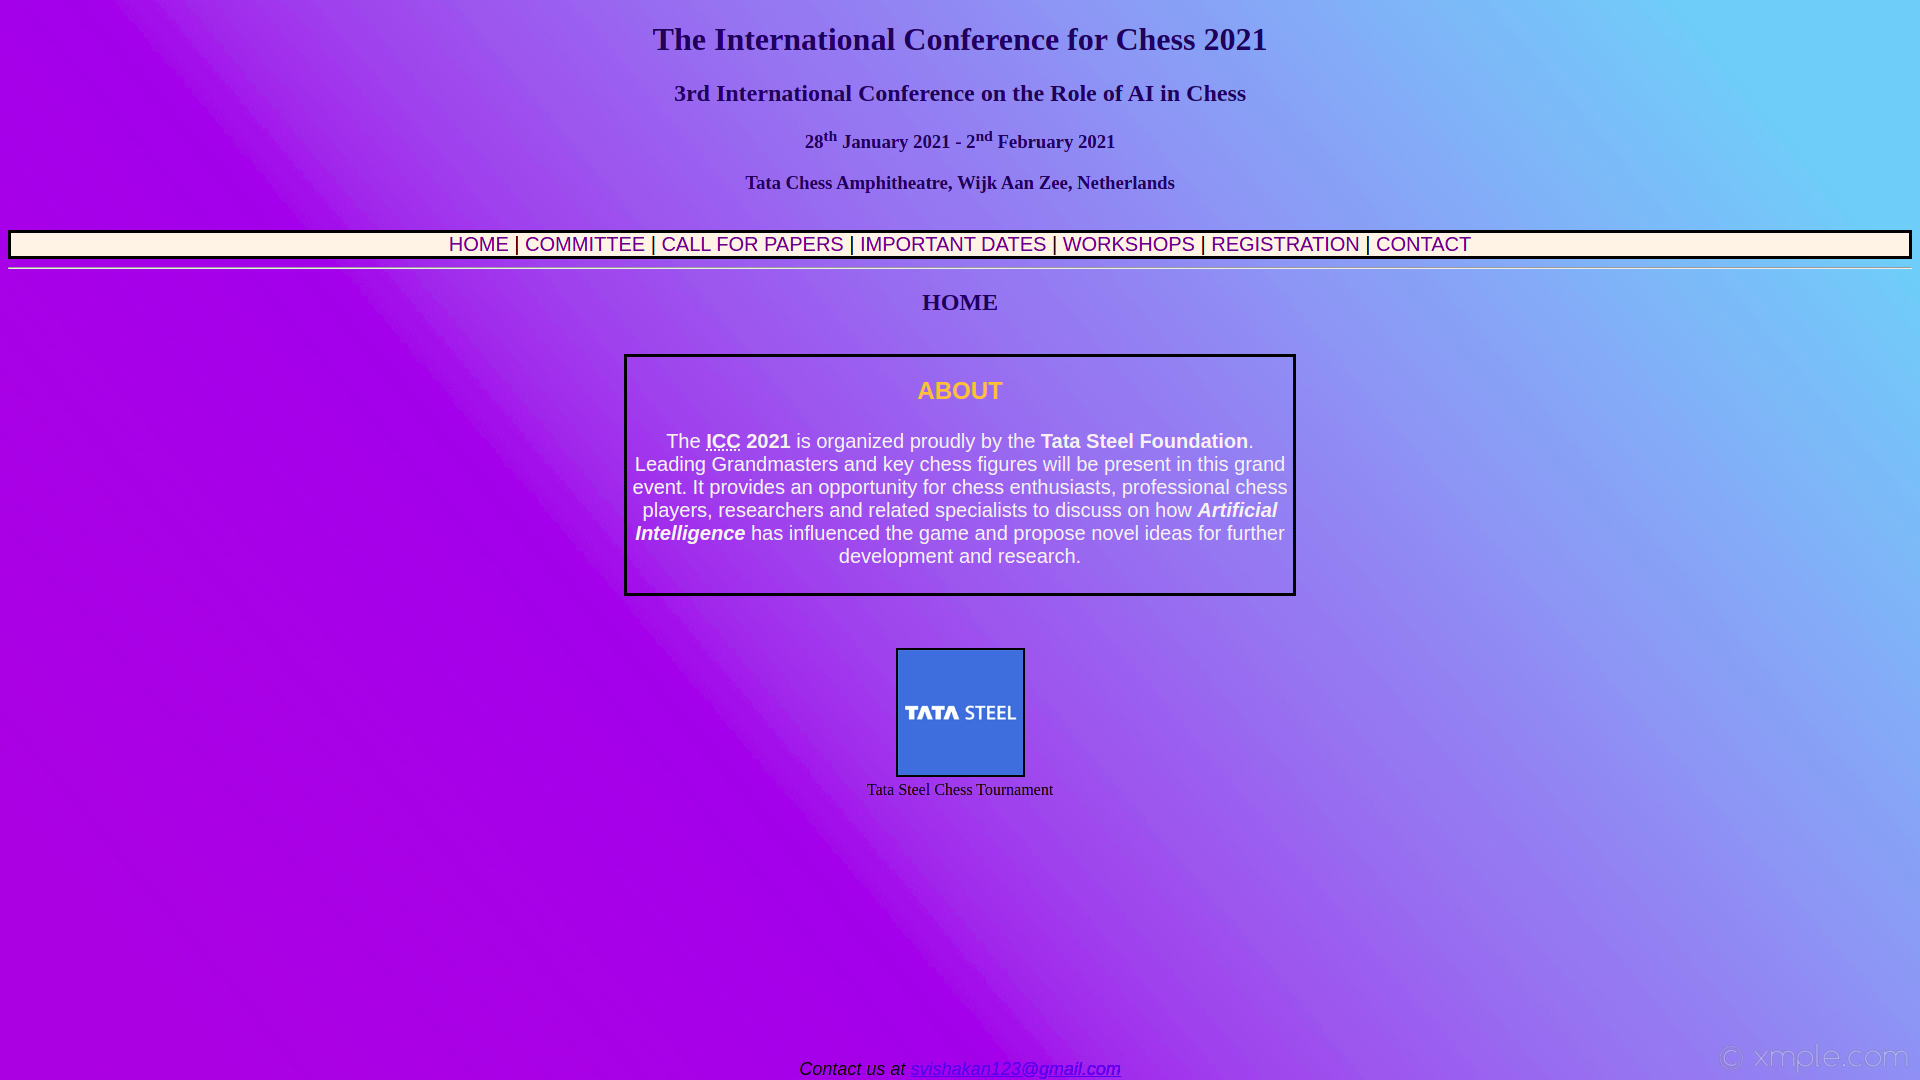
\includegraphics[scale = 0.25]{Output/Home.png}
\end{figure}

\newpage
\subsection*{\flushleft{Output - Committee Page:}}
\begin{figure}[h]
\centering
\caption{Browser Output: Committee Page.}
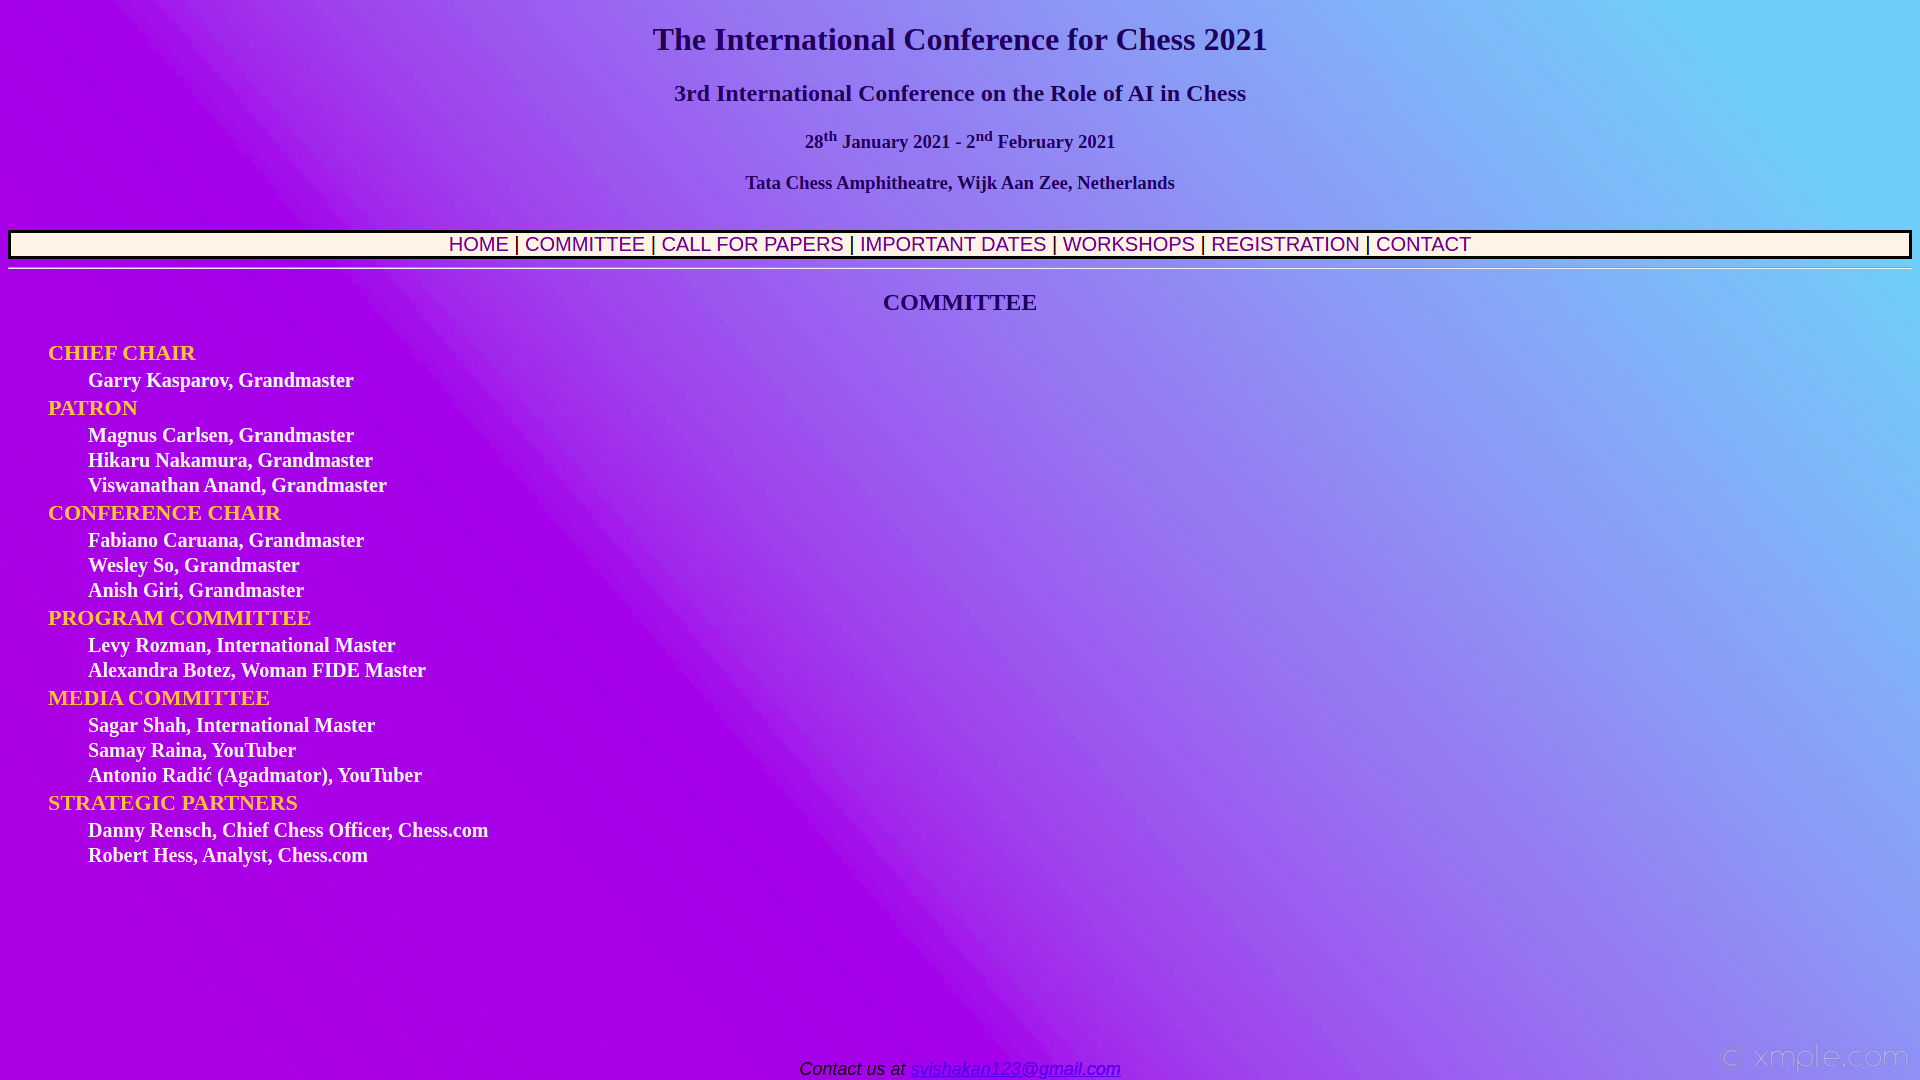
\includegraphics[scale= 0.25]{Output/Committee.png}
\end{figure}

\newpage
\subsection*{\flushleft{Output - Call For Papers Page:}}
\begin{figure}[h]
\centering
\caption{Browser Output: Call For Papers Page.}

\includegraphics[scale= 0.25]{Output/Papers.png}
\end{figure}

\newpage
\subsection*{\flushleft{Output - Important Dates Page:}}
\begin{figure}[h]
\centering
\caption{Browser Output: Important Dates Page.}
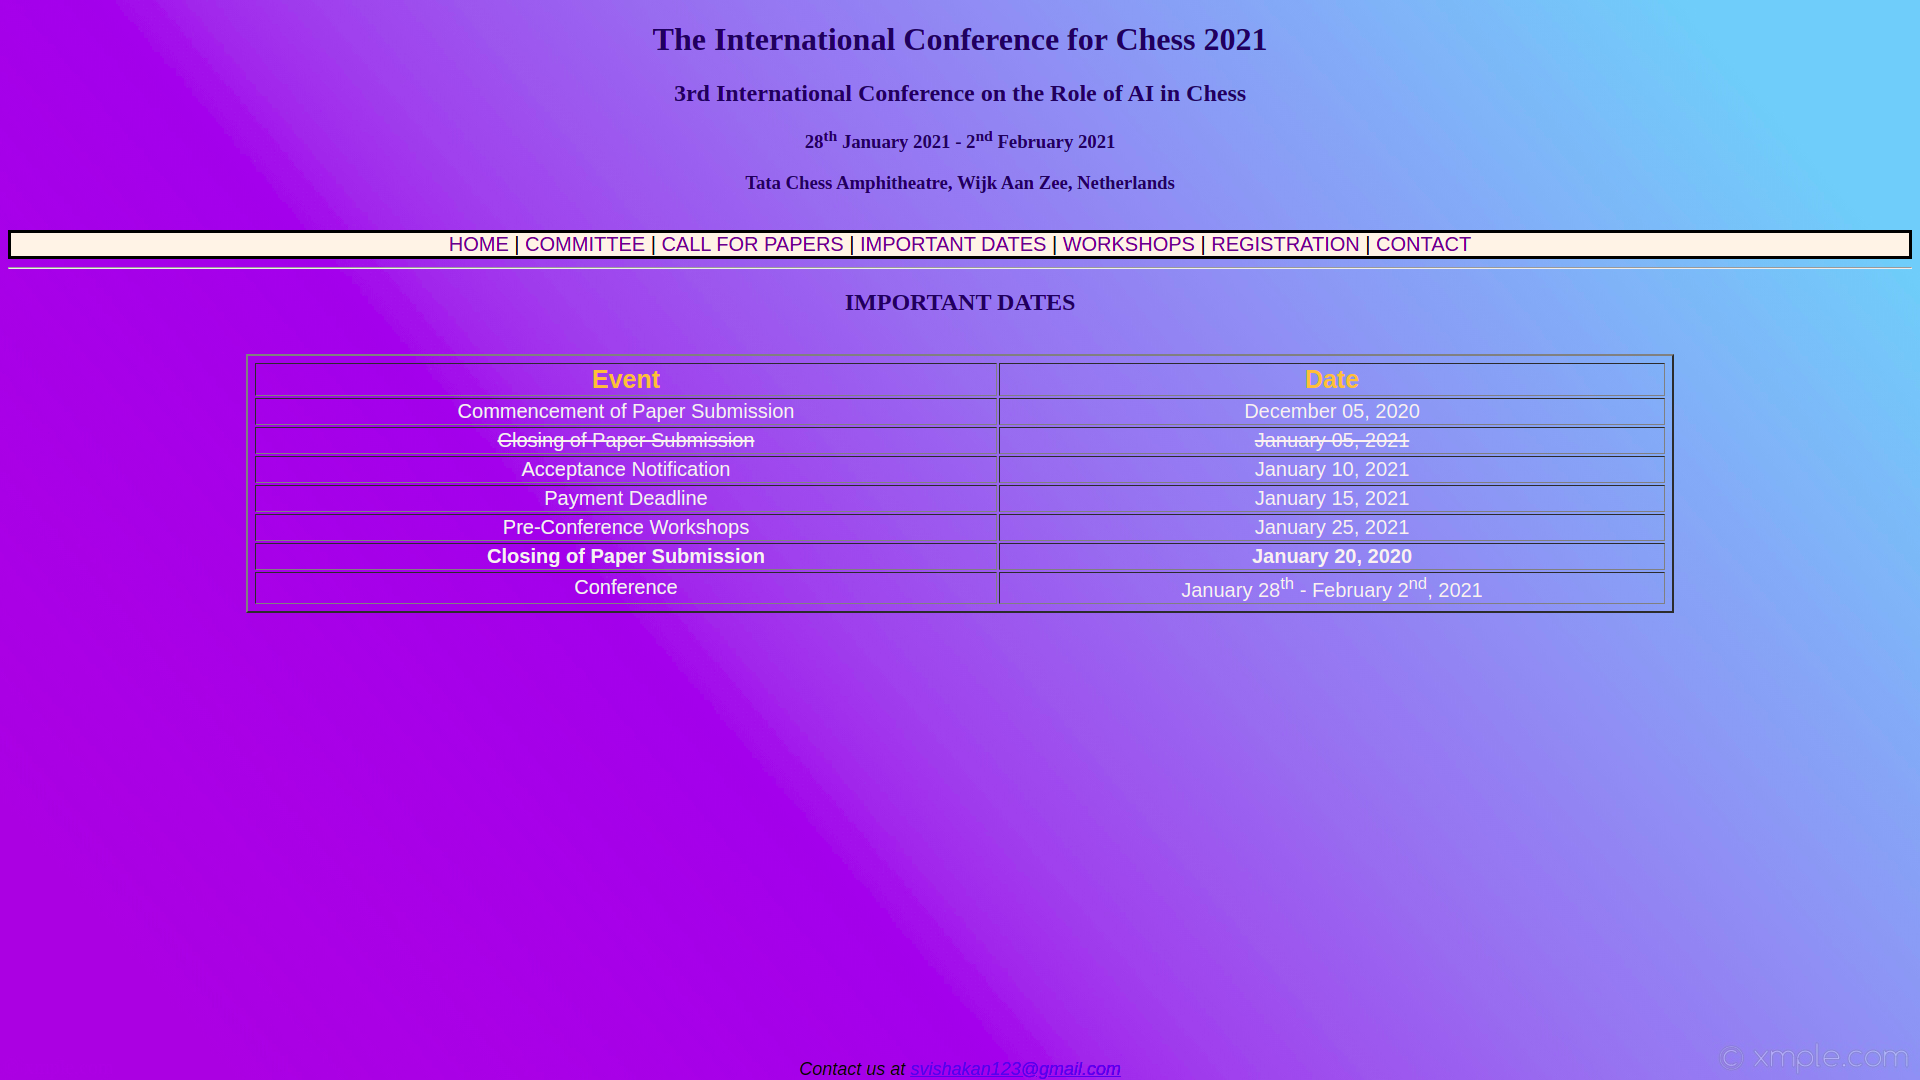
\includegraphics[scale= 0.25]{Output/Dates.png}
\end{figure}

\newpage
\subsection*{\flushleft{Output - Workshops Page:}}
\begin{figure}[h]
\centering
\caption{Browser Output: Workshops Page.}
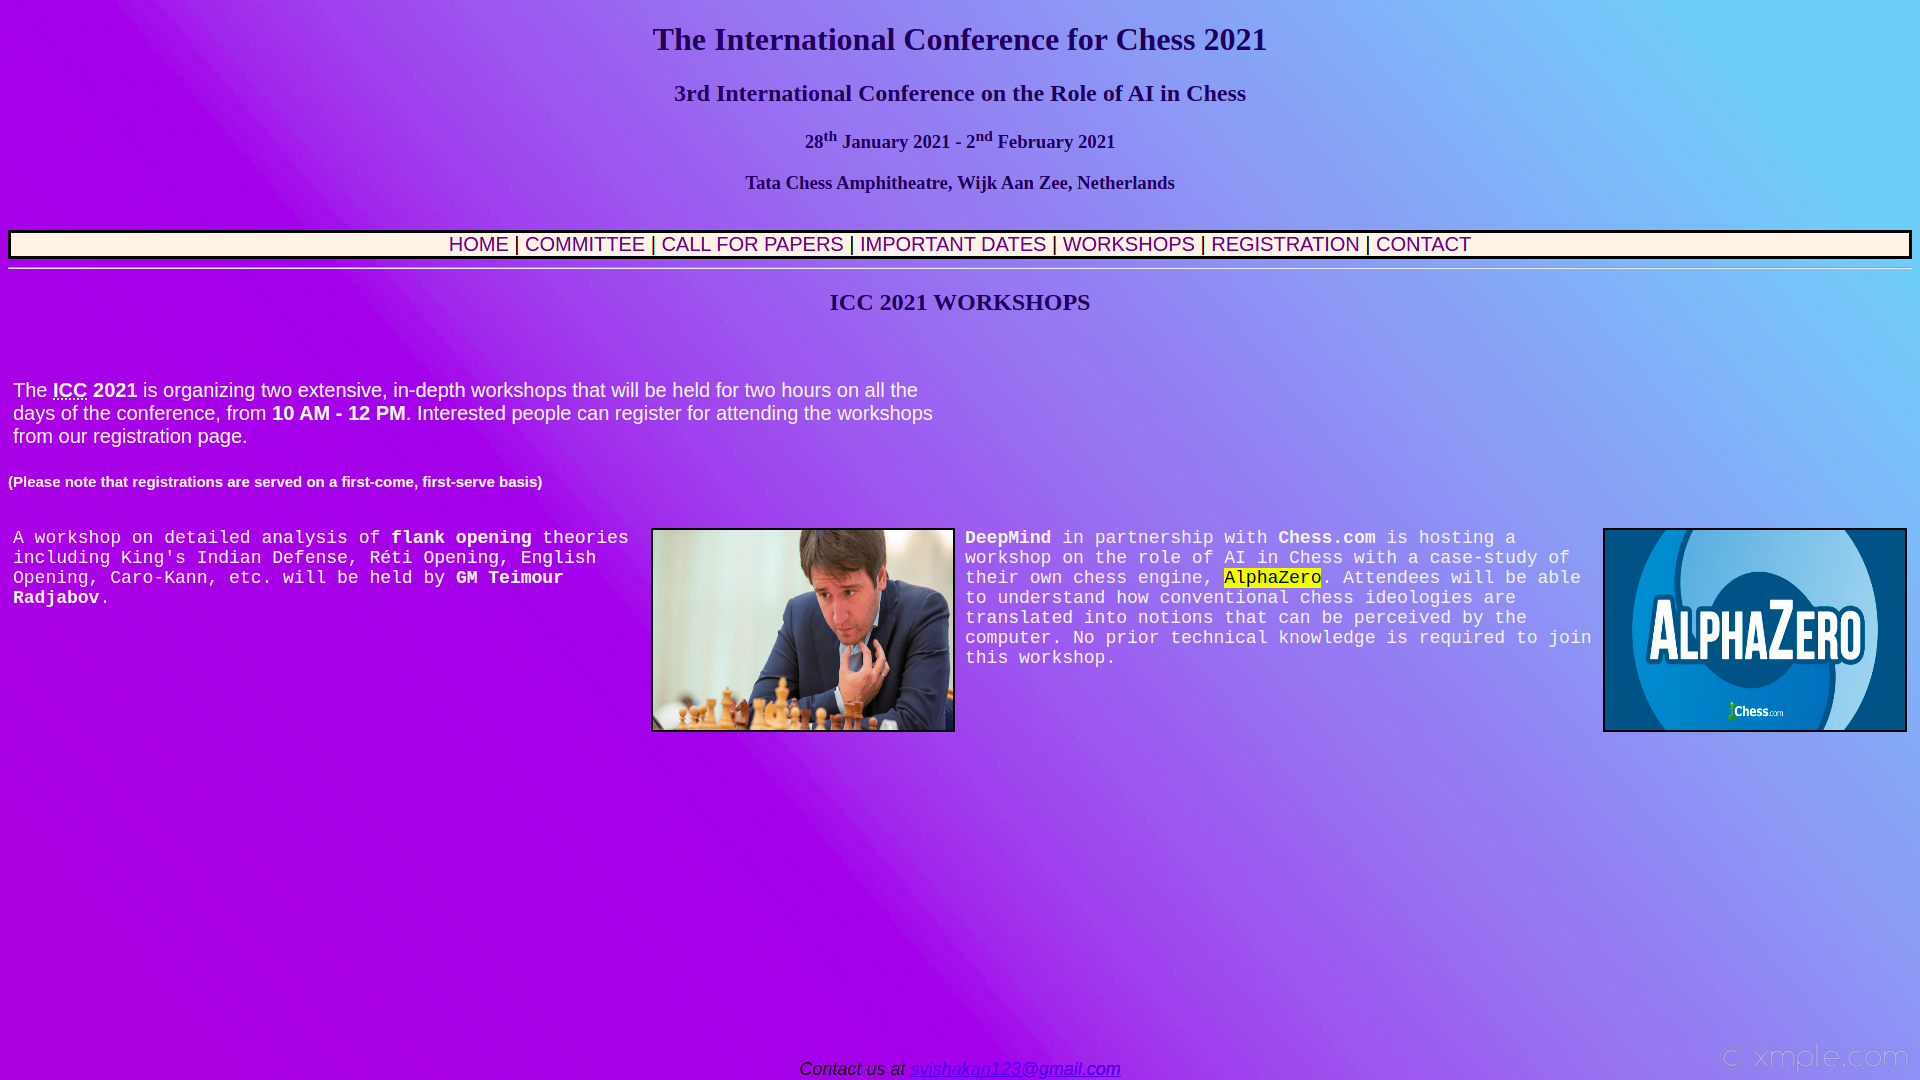
\includegraphics[scale= 0.25]{Output/Workshops.png}
\end{figure}

\newpage
\subsection*{\flushleft{Output - Registration Page:}}
\begin{figure}[h]
\centering
\caption{Browser Output: Registration Page.}
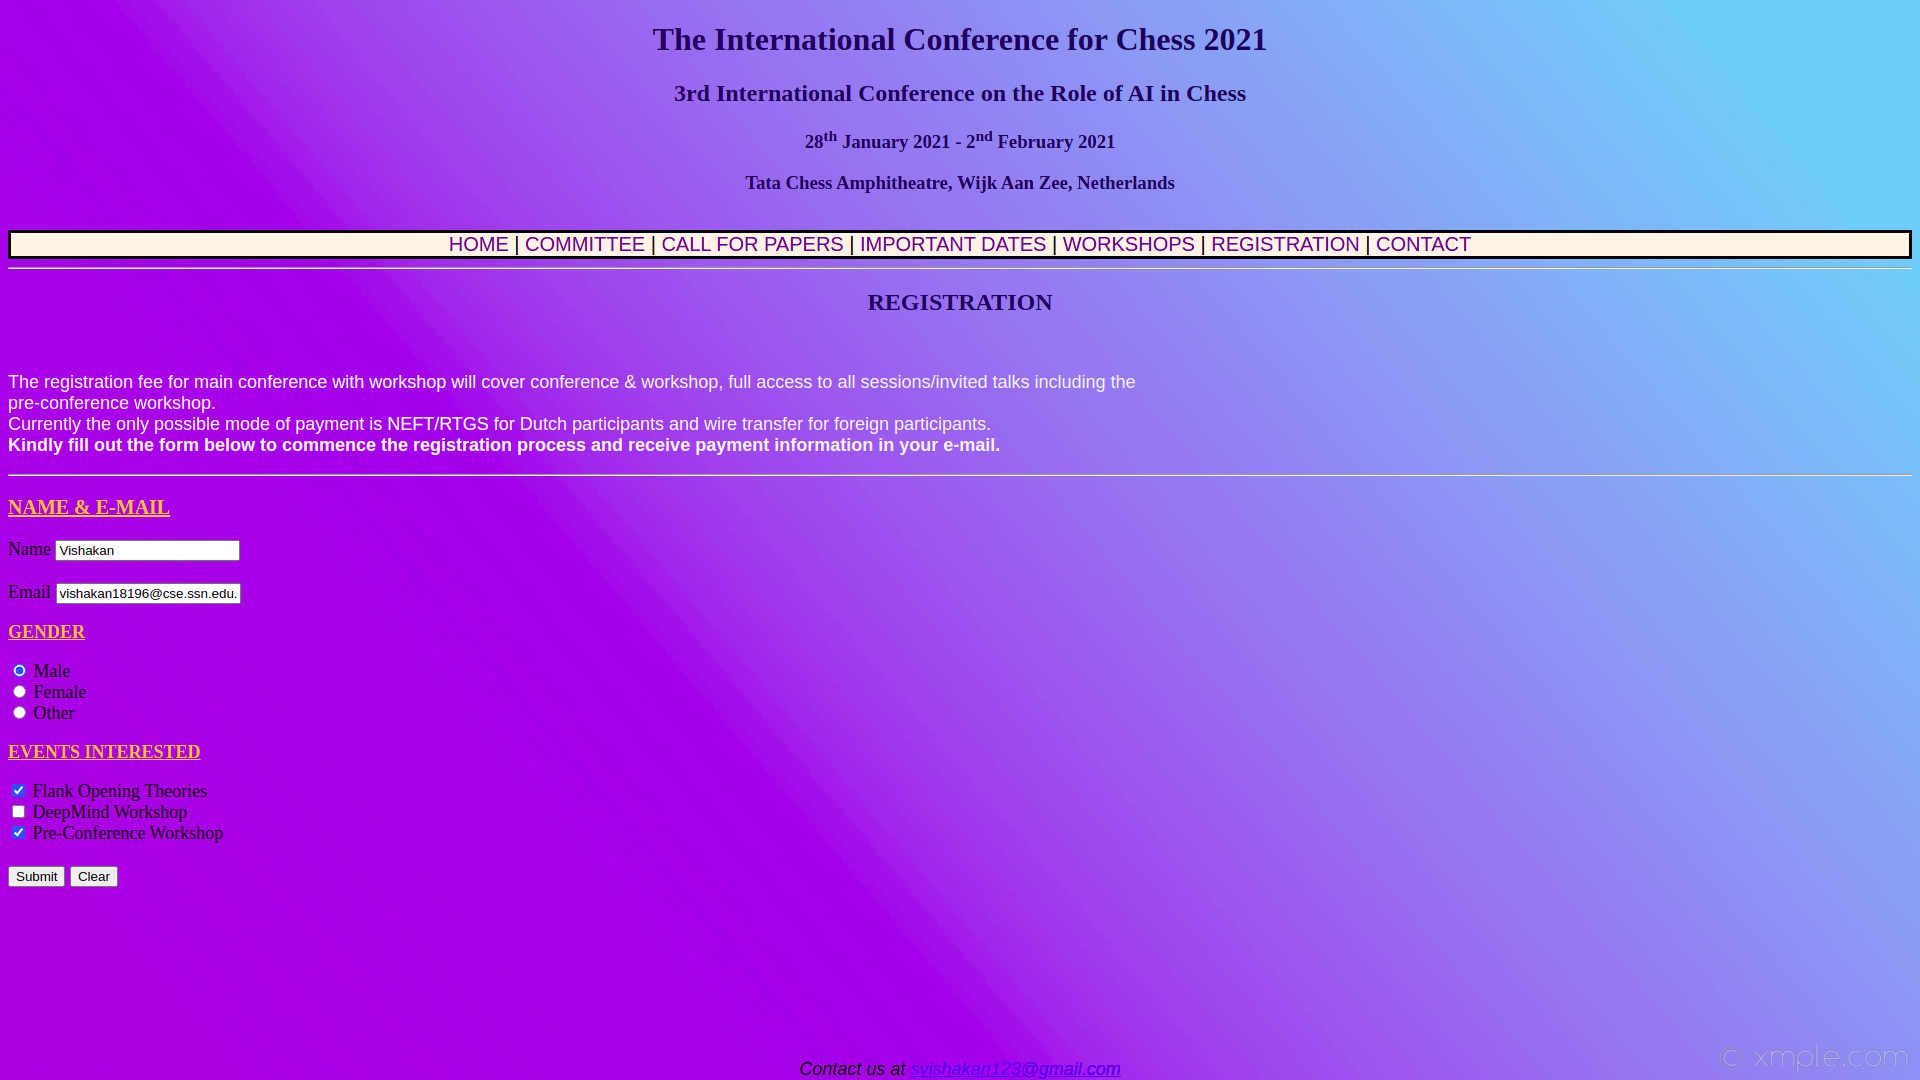
\includegraphics[scale= 0.25]{Output/Registration.png}
\end{figure}

\newpage
\subsection*{\flushleft{Output - Contact Page:}}
\begin{figure}[h]
\centering
\caption{Browser Output: Contact Page.}
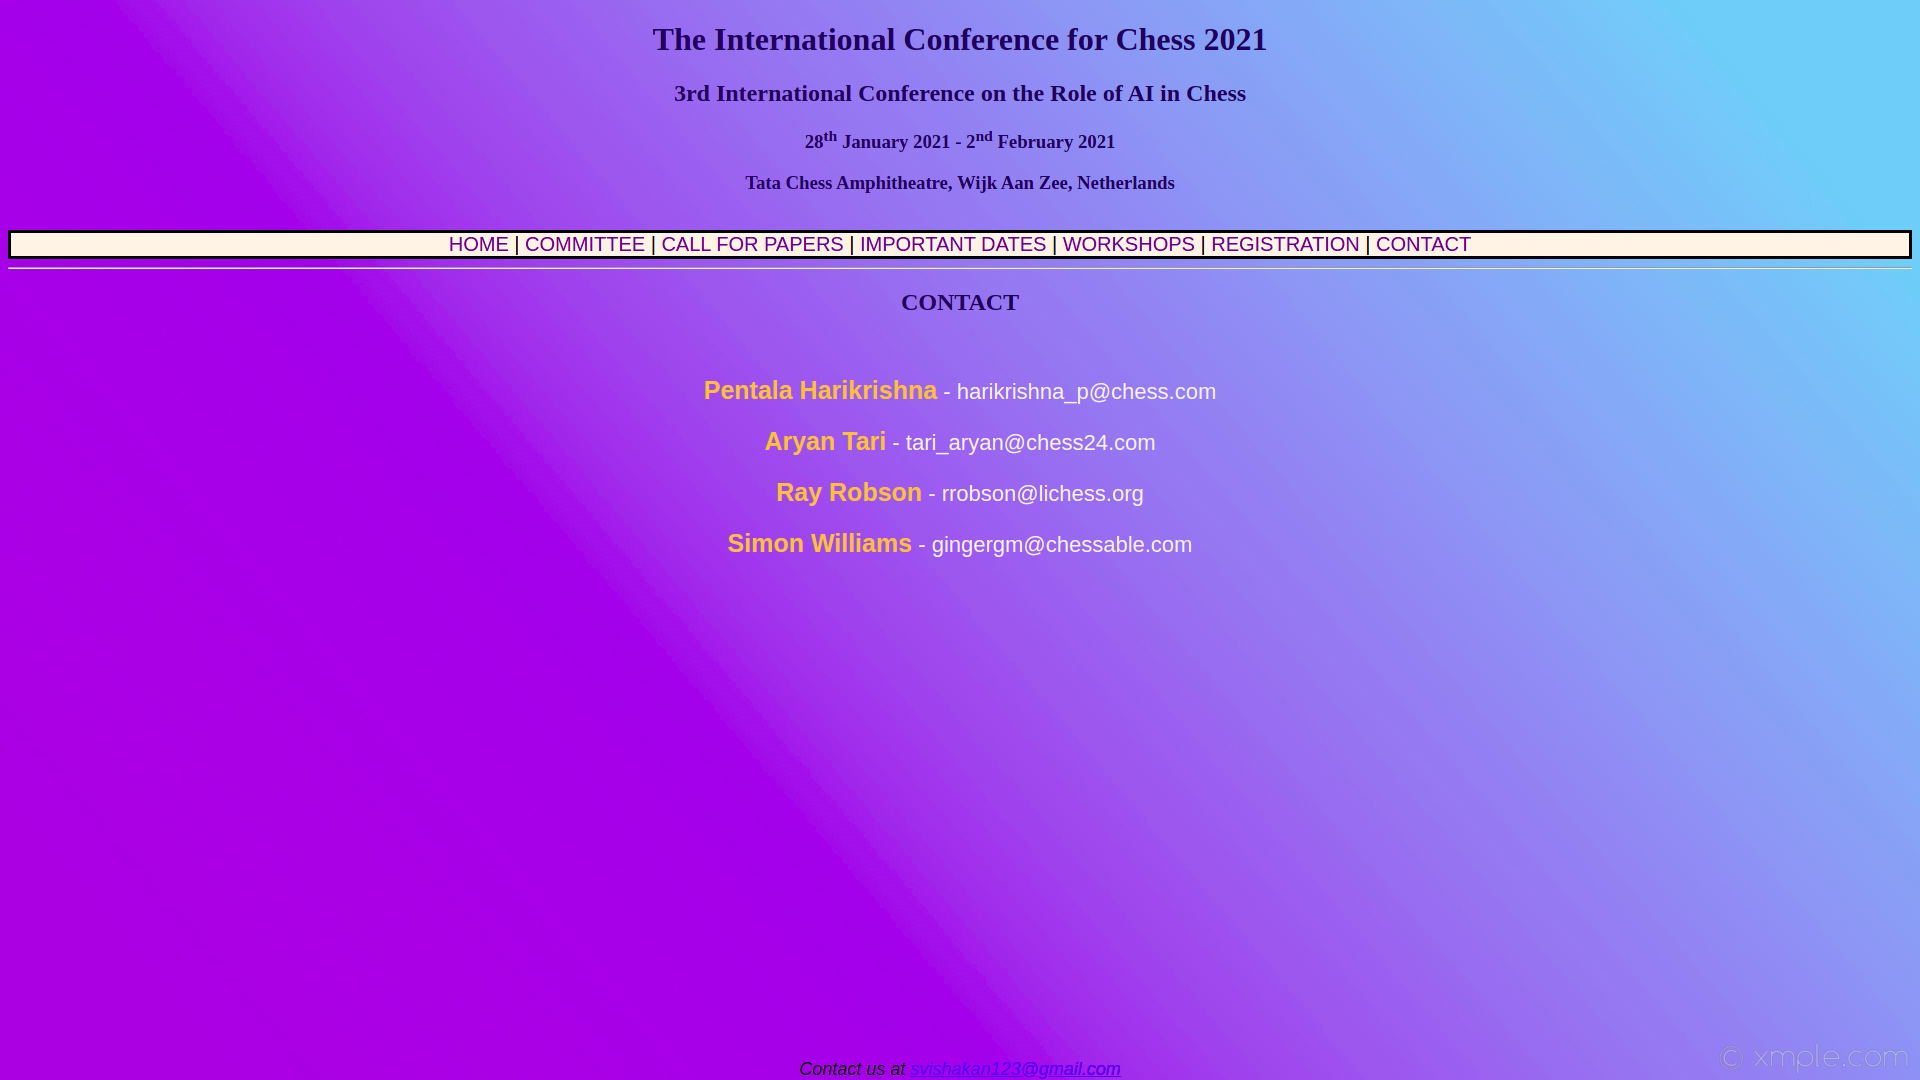
\includegraphics[scale= 0.25]{Output/Contact.png}
\end{figure}

%Learning Outcome
\newpage
\subsection*{\flushleft{Learning Outcome:}}
\begin{itemize}

\item From the experiment, I learnt to implement basic HTML5 tags.
\item I learnt about basic attributes for the HTML5 tags that I used in the experiment.
\item I learnt the syntax of HTML5.
\item I learnt about using HTML5 Anchor Tag to link to another webpage.
\item I was able to implement the addition of images and captions in a webpage.
\item I learnt how to create tables and lists in HTML5.
\item I learnt about basic form creation using HTML5.
\item I learnt and implemented various semantic tags of HTML5.
\item I learnt how to perform basic formatting of HTML5 tags to enhance the look and feel of the webpage.
\item I learnt about text formatting tags like strong, emphasis, superscript, subscript and strikethrough tags.

\end{itemize}

\end{document}
